\documentclass[twocolumn]{report}
\usepackage[margin=1in]{geometry}
\usepackage{amsmath}
\usepackage{amssymb}
\usepackage{subfiles}

\title{ENGT 3652 Project 5:\\*CNC Lathe-Bishop}
\author{Leomar Dur\'an}
\date{${25}^{\text{th}}$ April 2023}

\usepackage{pdflscape}
\usepackage{graphicx}
\usepackage{minted}
\newcommand*\gcode{lib/pygments/gcodelexer.py:GcodeLexer -x}

\usepackage[final]{pdfpages}
%\write18{
%    % the manual gcode for CNC Simulator in two columns
%    pdflatex gcode-cam
%}
% usage: \includepdf[pages=2-,pagecommand={}]{gcode-cam.pdf}

%\usepackage[final]{pdfpages}
%% compile the subfiles
%\write18{
%    % the manual gcode in two columns
%    pdflatex gcode-manual
%}
%\write18{
%    % the manual gcode for CNC Simulator in two columns
%    pdflatex gcode-manual-for_cnc_simulator
%}
%\write18{
%    % the manual MasterCAM-generated gcode in two columns
%    pdflatex gcode-cam
%}

\begin{document}

\maketitle

\onecolumn
    \chapter{Original drawing}
    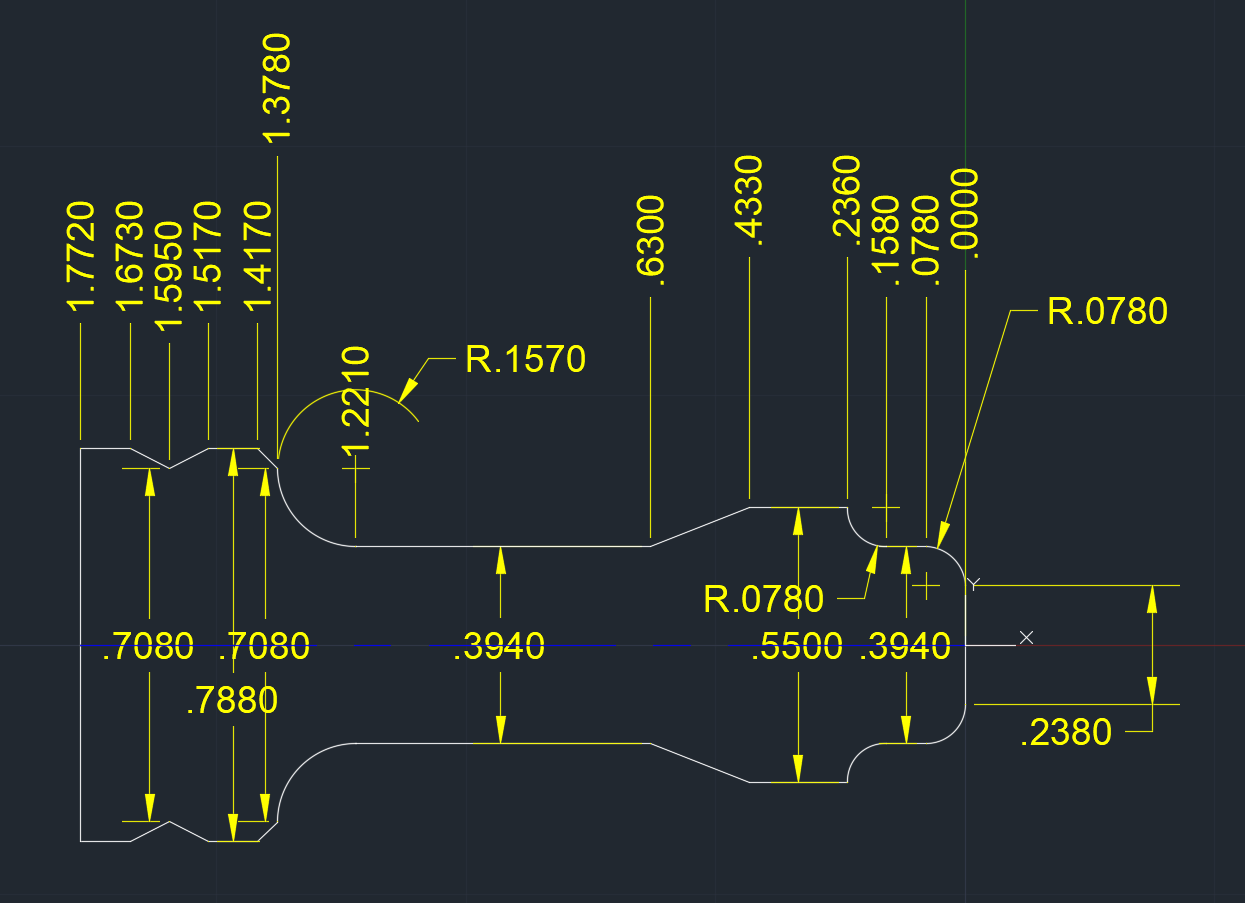
\includegraphics[width=\textwidth]{Bishop - The path_pptx/ppt/media/image1.png}
\twocolumn

%\chapter{Path}/
\onecolumn
    \addtocounter{chapter}{1}
    \includepdf[landscape,pages=-,pagecommand={}]{Bishop - The path_pptx.pdf}
\twocolumn

\chapter{Manual Gcode}
\inputminted[breaklines]\gcode{src/bishopManual.nc}

\chapter{Plot of manual Gcode in NCViewer}
\onecolumn
    \begin{landscape}
    % this image has a lower portrait aspect ratio than a page, so use height for reference
    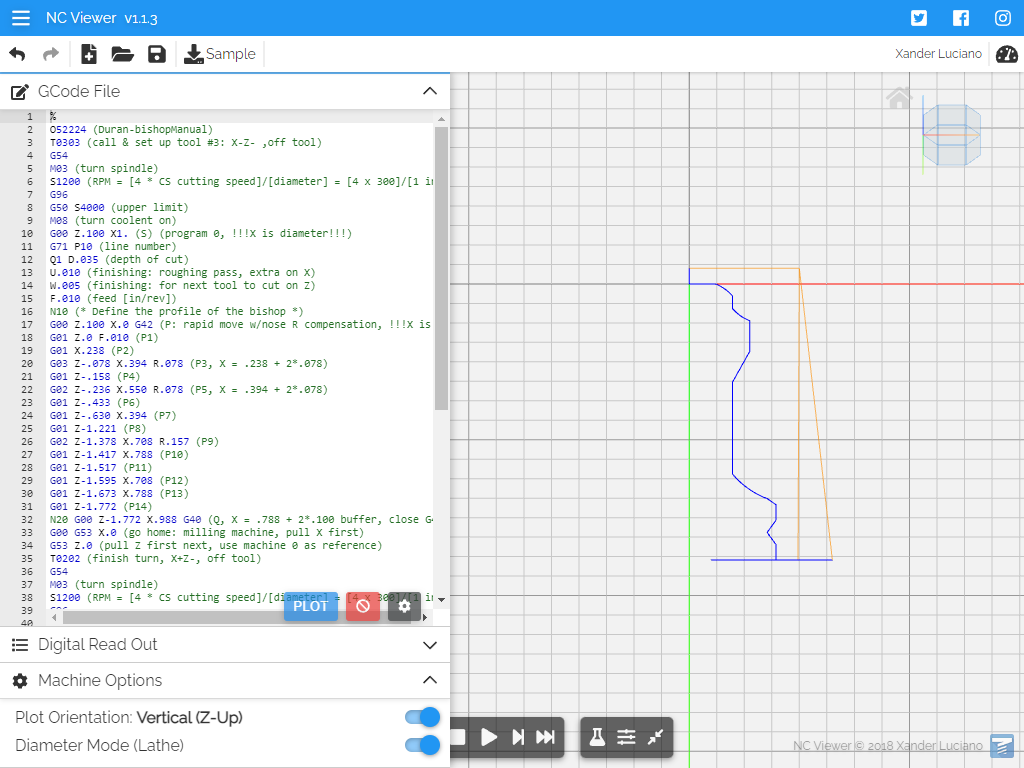
\includegraphics[height=\textheight]{img/prj05-manual-gcode-ncviewer-plot-xz.png}
    \end{landscape}
\twocolumn

\chapter{Manual Gcode, edited for CNC Simulator}
\inputminted[breaklines]\gcode{src/bishopManualForCncSim.nc}

\chapter{Result of manual Gcode for CNC Simulator}
\onecolumn
    \begin{landscape}
        \null\vfill
        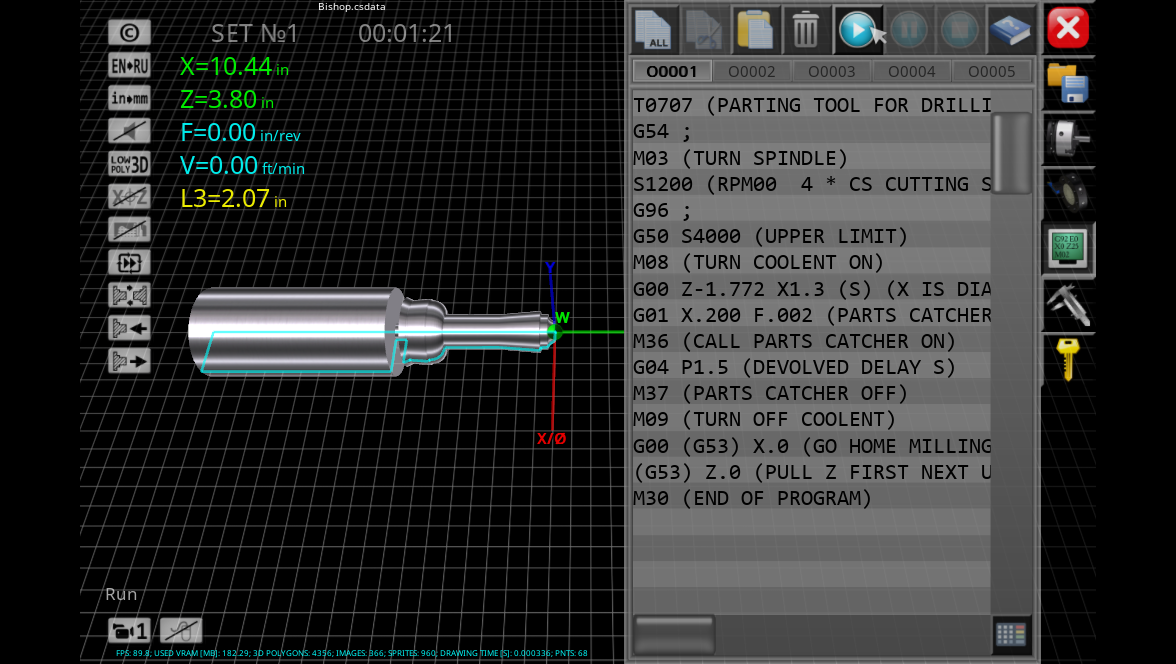
\includegraphics[width=\linewidth]{img/prj05-cnc_simulator_result.png}
        \vfill
    \end{landscape}
\twocolumn

\chapter{Verification of operations in Mastercam}
\onecolumn
    \begin{landscape}
        \vfill
        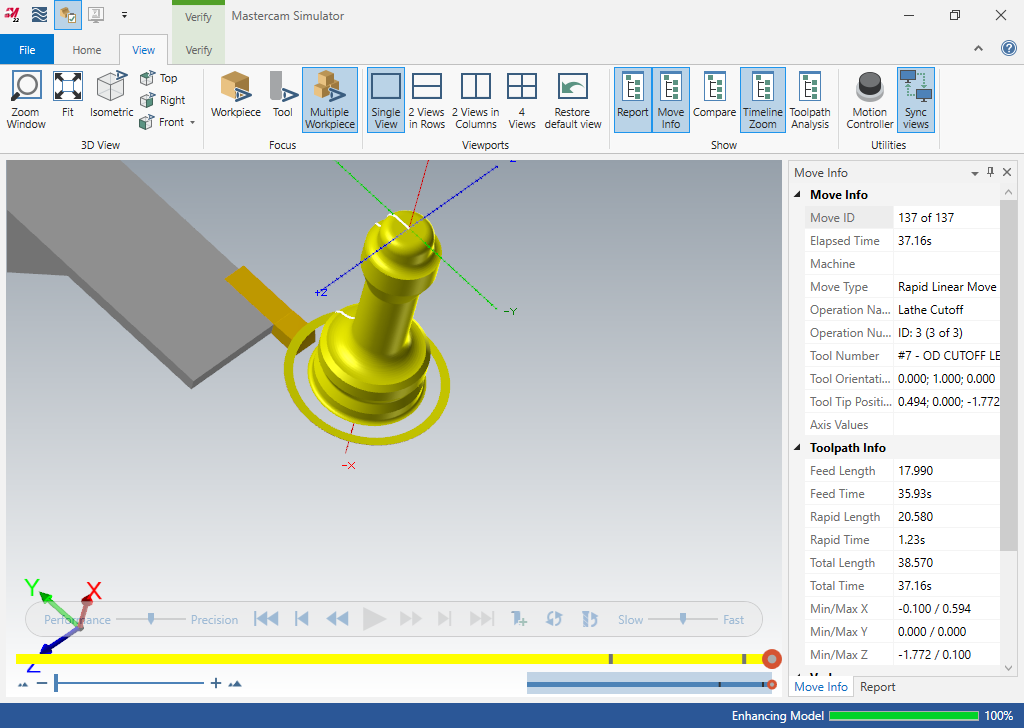
\includegraphics[width=\linewidth]{img/prj05-mastercam_simulator-verification.png}
        \vfill
    \end{landscape}
\twocolumn

\chapter{The MasterCAM generated Gcode}
\inputminted[breaklines]\gcode{src/bishopFromCam.nc}

\chapter{Plot of MasterCAM-generated Gcode in NCViewer}
\onecolumn
    \begin{landscape}
    % this image has a lower portrait aspect ratio than a page, so use height for reference
    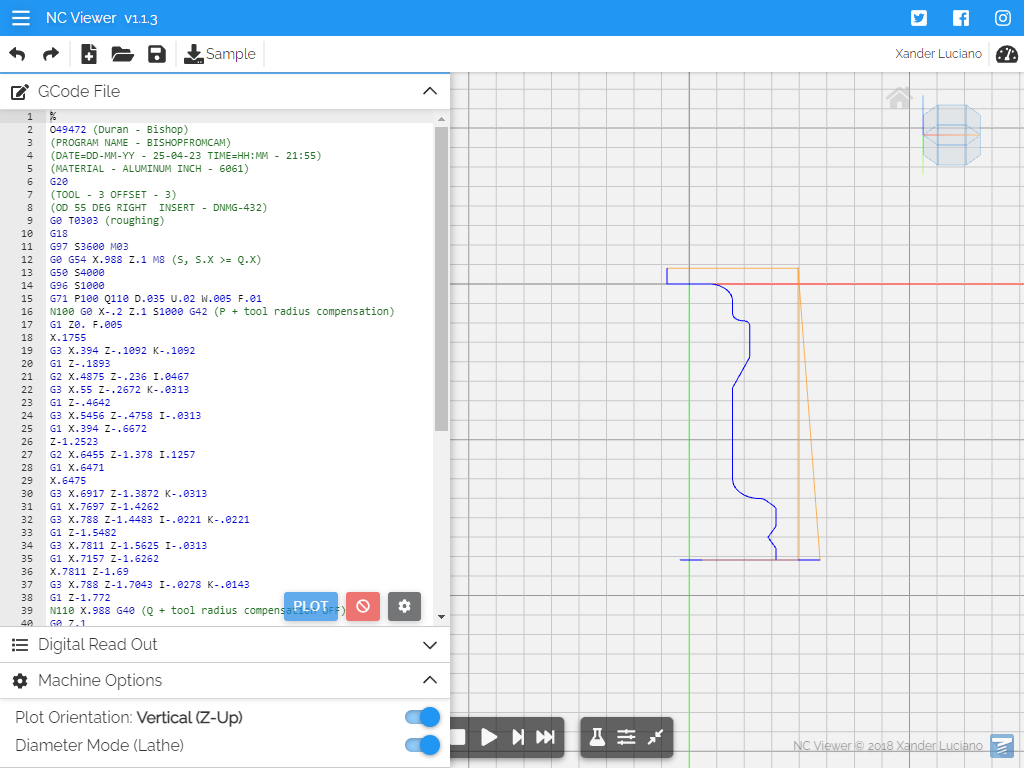
\includegraphics[height=\textheight]{img/prj05-cam-gcode-ncviewer-plot-xz.png}
    \end{landscape}
\twocolumn

\onecolumn
    \chapter{The machined part}
    \null\vfill
    \centering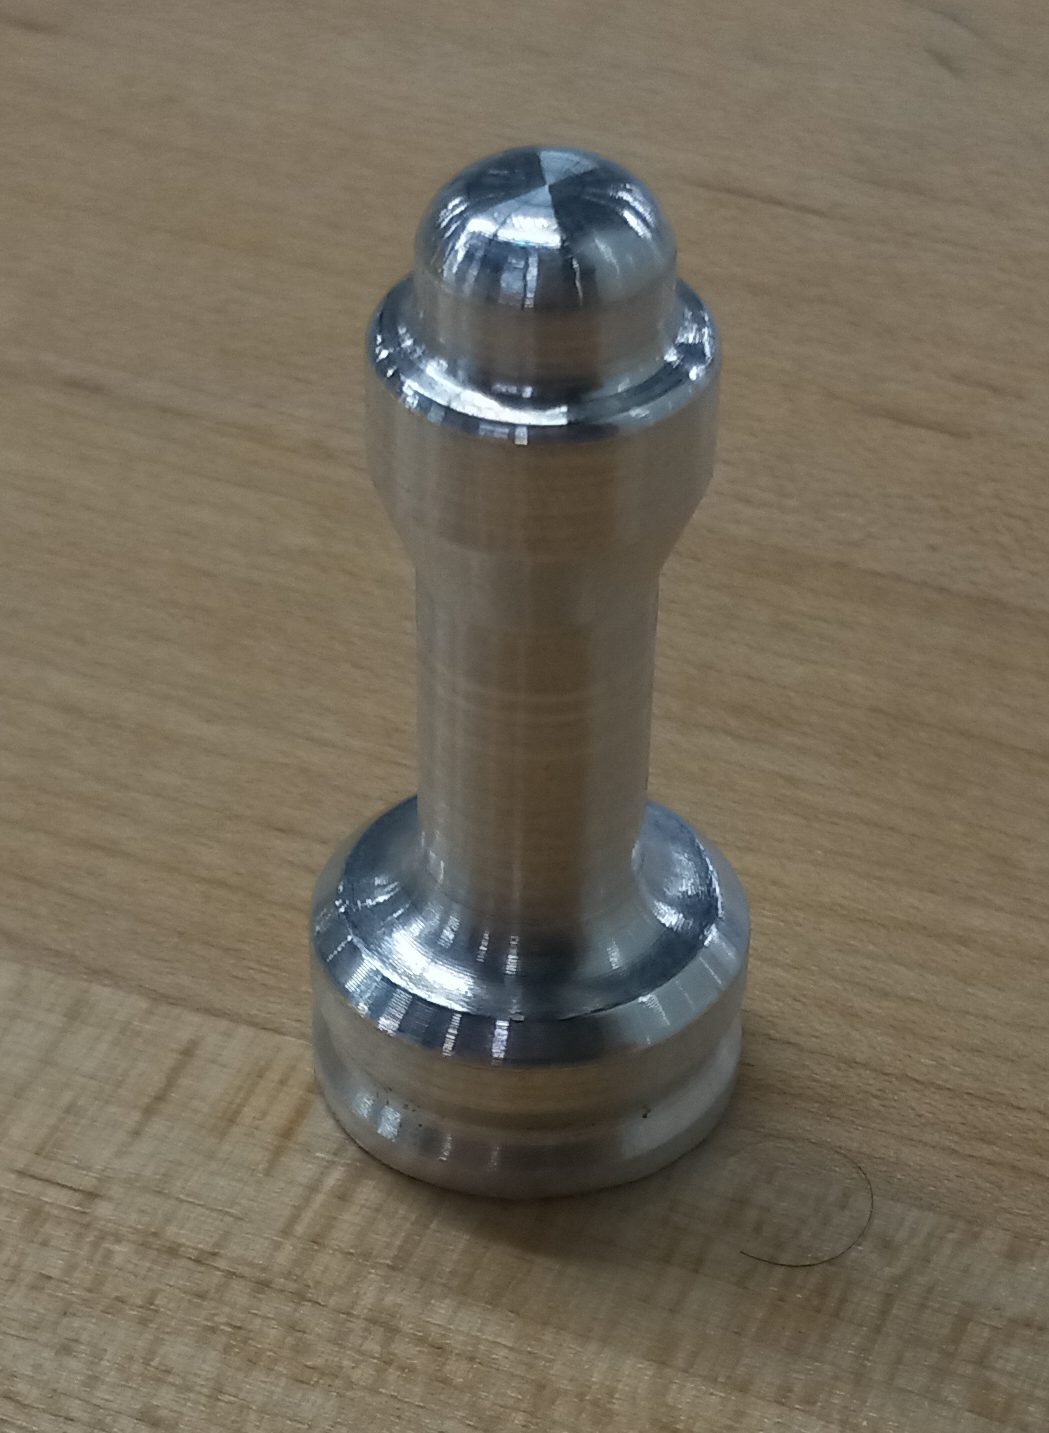
\includegraphics[width=0.7\linewidth]{img/machined-05-cnc_lathe-bishop.png}
    \vfill
\twocolumn

\end{document}
